\section{Introduction}\label{sec:intro}

We will denote by $|a-b|_X$ the distance between points $a$ and $b$ in the metric space $X$.

\parbf{Tree comparison.}
Fix a tree $T$ with $n$ vertexes.

Let $(a_1,\dots a_n)$ be a point array in a metric space $X$ labeled by the vertexes of $T$.
We say that $(a_1,\dots a_n)$  satisfies the \emph{$T$-tree comparison} if there is a point array $(\~a_1,\dots, \~a_n)$ in the Hilbert space $\HH$ such that 
\[|\~a_i-\~a_j|_\HH\ge|a_i-a_j|_X\]
for any $i$ and $j$ and equality holds if $a_i$ and $a_j$ are adjacent in $T$.

We say that a metric space $X$ satisfies the \emph{$T$-tree comparison} if 
every $n$-points array in $X$ satisfies the $T$-tree comparison.

Instead of the Hilbert space $\HH$, we may use an infinite dimensional sphere or an infinite dimensional hyperbolic space.
In this case it defines \emph{spherical} and \emph{hyperbolic} tree comparisons.

\begin{wrapfigure}{r}{27 mm}
\vskip-8mm
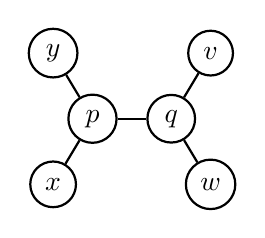
\begin{tikzpicture}[scale=1,
  thick,main node/.style={circle,draw,font=\sffamily\bfseries,minimum size=3mm}]
  \node[main node] (1) at (-1/2,-5/6) {$x$};
  \node[main node] (2) at (0,0){$p$};
  \node[main node] (3) at (-1/2,5/6){$y$};
  \node[main node] (4) at (3/2,5/6) {$v$};
  \node[main node] (5) at (1,0) {$q$};
  \node[main node] (6) at (3/2,-5/6) {$w$};

  \path[every node/.style={font=\sffamily\small}]
   (1) edge node[above]{}(2)
   (2) edge node[above]{}(3)
   (2) edge node[above]{}(5)
   (4) edge node[above]{}(5)
   (5) edge node[above]{}(6);
\end{tikzpicture}
\end{wrapfigure}

\parbf{Encoding of trees.}
To encode the labeled tree on the diagram, we will use notation $p/xy(q/vw)$.
It means that we choose $p$ as the root; 
$p$ has two children leaves $x$, $y$ and one child $q$ with two children leaves $v$ and $w$.
Taking another root for the same tree, we get different encodings, for example $q/vw(p/xy)$ or $x/(p/y(q/vw))$.

If we do not need the labeling of vertexes,
it is sufficient to write the number of leaves in the brackets;
this way we can write 2(2) instead of $p/xy(q/vw)$ since the root ($p$) has 2 leaves ($x$ and $y$) and yet another child ($q$) that has 2 leaves ($v$ and $w$).  
The same tree can be encoded as (1(2)) meaning that the root $x$ has no leaves, 
$p$ has 1 leaf $y$ and one child $q$ with 2 leaves $v$ and $w$.
Note that every vertex that is not the root and not a leaf corresponds to a pair of brackets in this notation.

Using the described notation, we could say that a metric space \emph{satisfies the 2(2)-tree comparison},  meaning that it satisfies the tree comparison on the diagram.
We could also say \emph{``applying the tree comparison for $p/xy(q/vw)$ ...''} meaning that we apply the comparison for these 6 points in a metric space labeled as on the diagram.

\parbf{Monopolar trees.}
A vertex of a tree of degree at least two will be called a \emph{pole}.

\begin{wrapfigure}{r}{21 mm}
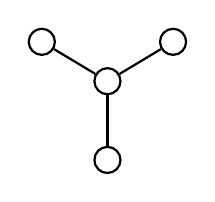
\begin{tikzpicture}[scale=1,
  thick,main node/.style={circle,draw,font=\sffamily\bfseries,minimum size=3mm}]

  \node[main node] (1) at (5/6,1) {};
  \node[main node] (2) at (0,3/2){};
  \node[main node] (3) at (10/6,3/2){};
  \node[main node] (4) at (5/6,0) {};

  \path[every node/.style={font=\sffamily\small}]
   (1) edge node[above]{}(2)
   (1) edge node[above]{}(3)
   (1) edge node[above]{}(4);
\end{tikzpicture}
\end{wrapfigure}

Recall that \emph{Alexandrov space} with nonnegative curvature is defined as a complete length space with \emph{nonnegative curvature in the sense of Alexandrov};
the latter is equivalent to the 3-tree comparison; that is, the comparison for the tripod-tree on the diagram. 

Using the introduced notation, the theorem on ($n$+1)-point comparison in \cite{AKP} can be restated the following way: \emph{If a complete length-metric space satisfies $3$-tree comparison, then it also satisfies $n$-tree comparison for every positive integer~$n$; in other words it satisfies all monopolar tree comparisons.}

\parbf{Bipolar comparison.}
The following theorem is proved in sections~\ref{sec:pivotal} and \ref{6-dipole};
it describes the comparisons for the bipolar trees 3(1) and 2(2) shown on the diagram.

\begin{center}
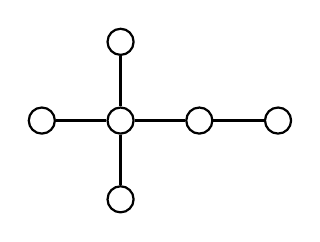
\begin{tikzpicture}[scale=1,
  thick,main node/.style={circle,draw,font=\sffamily\bfseries,minimum size=3mm}]

  \node[main node] (1) at (1,2) {};
  \node[main node] (2) at (1,0){};
  \node[main node] (3) at (1,1){};
  \node[main node] (4) at (0,1) {};
  \node[main node] (5) at (3,1) {};
  \node[main node] (6) at (2,1) {};

  \path[every node/.style={font=\sffamily\small}]
   (1) edge node[above]{}(3)
   (2) edge node[above]{}(3)
   (3) edge node[above]{}(6)
   (4) edge node[above]{}(3)
   (5) edge node[above]{}(6);
\end{tikzpicture}
\hskip30mm
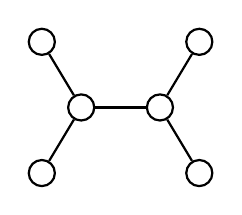
\begin{tikzpicture}[scale=1,
  thick,main node/.style={circle,draw,font=\sffamily\bfseries,minimum size=3mm}]

  \node[main node] (1) at (0,0) {};
  \node[main node] (2) at (1/2,5/6){};
  \node[main node] (3) at (0,10/6){};
  \node[main node] (4) at (2,0) {};
  \node[main node] (5) at (3/2,5/6) {};
  \node[main node] (6) at (2,10/6) {};

  \path[every node/.style={font=\sffamily\small}]
   (1) edge node[above]{}(2)
   (2) edge node[above]{}(3)
   (2) edge node[above]{}(5)
   (4) edge node[above]{}(5)
   (5) edge node[above]{}(6);
\end{tikzpicture}
\end{center}

\begin{thm}{Theorem}\label{thm:3(1)+2(2)}
A complete Riemannian manifold has nonnegative sectional curvature if and only if it satisfies 3(1)-tree (or 2(2)-tree) comparison.
\end{thm}

{

\begin{wrapfigure}{r}{32 mm}
\vskip-2mm
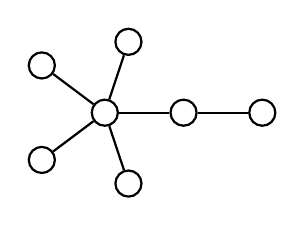
\begin{tikzpicture}[scale=1,
  thick,main node/.style={circle,draw,font=\sffamily\bfseries,minimum size=3mm}]

  \node[main node] (0) at (.3,.9){};
   \node[main node] (1) at (-.8,-.6){};
  \node[main node] (2) at (.3,-.9){};
  \node[main node] (3) at (0,0){};
  \node[main node] (4) at (-.8,.6){};
  \node[main node] (5) at (2,0){};
  \node[main node] (6) at (1,0){};

  \path[every node/.style={font=\sffamily\small}]
     (0) edge node[above]{}(3)
   (1) edge node[above]{}(3)
   (2) edge node[above]{}(3)
   (3) edge node[above]{}(6)
   (4) edge node[above]{}(3)
   (5) edge node[above]{}(6);
\end{tikzpicture}
\end{wrapfigure}

The proof is given in Section~\ref{6-dipole}.

\bigskip

The following theorem gives a description of Riemannian manifolds satisfying 4(1)-tree comparison (the 4(1)-tree is shown on the diagram).
Let us first define CTIL Riemannian manifolds (CTIL stands for \emph{convexity of tangent injectivity locus}).

}

Let $M$ be a Riemannian manifold and $p\in M$.
The subset of tangent vectors $v\in\T_p$ such that there is a minimizing geodesic $[p\,q]$ in the direction of $v$ with length $|v|$ will be denoted as $\overline{\TIL}_p$.
The interior of $\overline{\TIL}_p$ is denoted by $\TIL_p$; it is called \emph{tangent injectivity locus} at $p$.
If at $\TIL_p$ is convex for any $p\in M$, then $M$ is called CTIL.

For a function $f$ defined on an open convex set of Euclidean space we write 
$f''\le \lambda$ if for any unit-speed geodesic $\gamma$ the function
\[t\mapsto f\circ\gamma(t)-\tfrac\lambda2\cdot t^2\]
is a concave real-to-real function.

\begin{thm}{Main theorem}\label{thm:convexity}
If a complete Riemannian manifold $M$ satisfies $4(1)$-tree comparison, then it is CTIL and the following two conditions hold:
\begin{enumerate}[(i)]
\item\label{thm:convexity:convexity} For any $p,q\in M$, we have $f''\le 1$, where $f$ is the function $f\: \TIL_p\to \RR$ defined by
\[f(v)=\tfrac12\cdot\dist_q^2\circ\exp_p(v).\] 
\item\label{thm:convexity:MTW} For any point $p\in M$ and any three tangent vectors 
$W\in \TIL_p$, $X,Y\in \T_p$, we have
\[\frac{\partial^4}{\partial^2s\,\partial^2t}\left|\exp_p(s\cdot X)-\exp_p(W+t\cdot Y)\right|_M^2\le 0\eqlbl{eq:MTW}\]
at $t=s=0$.
\end{enumerate}


Moreover, if one of the conditions (\ref{thm:convexity:convexity}) or (\ref{thm:convexity:MTW}) holds in a CTIL Riemannian manifold $M$, then $M$ satisfies all bipolar comparisons; that is, the $m(n)$-tree comparison holds for any $m$ and $n$.
\end{thm}

The part of theorem related to the condition (\textit{\ref{thm:convexity:convexity}}) is proved in Section~\ref{convexity}.
The equivalence of the conditions (\textit{\ref{thm:convexity:convexity}}) and (\textit{\ref{thm:convexity:MTW}}) for CTIL manifolds is proved in Section~\ref{MTW+}.
These proofs and the proof of Theorem~\ref{thm:3(1)+2(2)} are essentially independent; a possible generalization to length-metric spaces is discussed in the final remarks.


Note that theorems \ref{thm:3(1)+2(2)} and \ref{thm:convexity} do not provide descriptions of manifolds only for the following two bipolar trees: 3(2) and 3(3).

A Riemannian manifold $M$ is called MTW if inequality \ref{eq:MTW} holds for any $p\in M$ and all triples of vectors $W\in \TIL_p$, $X,Y\in \T_p$ with an additional assumption $X\perp Y$.
The condition (\textit{\ref{thm:convexity:MTW}}) in the theorem is stronger since it does not require orthogonality; this condition is named MTW$^{\not\perp}$ in \cite{FRV-Nec+Suf}.

The MTW condition is named for Xi-Nan Ma, Neil Trudinger and Xu-Jia Wang who introduced it in \cite{MTW};
an important step in the understanding MTW was made by Grégoire Loeper in~\cite{loeper}.
Below we describe a connection between MTW and the so called \emph{transport continuity property}, briefly TCP.

A compact Riemannian manifold $M$ is called TCP 
if for any two regular measures with density functions bounded away from zero and infinity the generalized solution of Monge--Amp\`{e}re equation provided by optimal transport 
is a genuine (continuous) solution.

MTW turns out to be a necessary condition for TCP.
In \cite{FRV-Nec+Suf}, 
Alessio Figalli, 
Ludovic Rifford 
and C\'edric Villani showed that
a strict version of CTIL and MTW provides a sufficient condition for TCP.
From the proof of Theorem~\ref{thm:convexity} it is evident that spherical 4(1)-tree comparison implies the strict version of MTW; in particular, we get the following:

\begin{thm}{Corollary}
Any Riemannian manifold satisfying spherical 4(1)-tree comparison is TCP.
\end{thm}

Note that the identity $s''\equiv1$ holds for the function $s\:v\mapsto\tfrac12\cdot|v|^2$ defined on $\TIL_p$.
Therefore the condition $f''\le 1$ in (\textit{\ref{thm:convexity:convexity}}) is equivalent to 
concavity of the function $h\zz=f-s$.
The following proposition gives a description of the MTW condition via convexity of superlevel set of $h$.
Essentially, this proposition is just a reformulation of a synthetic description of MTW given by C\'edric Villani \cite[Proposition 2.6]{MTW+CTIL}.
(Our formulation can be proved by recursive application of Villani's description and Villani's description follows immideately from our fromulation.) 
The proof can be also obtained by a straightforward modification of the proof of Theorem~\ref{thm:convexity}.

\begin{thm}{Proposition}\label{prop:convexity}
A complete CTIL Riemannian manifold $M$ is MTW if and only if 
for any $p,q\in M$, the function $h\: \TIL_p\to \RR$ defined by
\[h(v)=\tfrac12\cdot(\dist_q^2\circ\exp_p(v)-|v|^2)\] 
has convex superlevel sets; that is, the set
\[\set{v\in\TIL_p}{h(v)> C}\]
is convex for any $C\in\RR$.
\end{thm}


\parbf{All tree comparisons.}
Recall that a map $f\:W\to X$ between metric spaces is called \emph{submetry} if for any $w\in W$ and $r\ge 0$, we have 
\[f[B(w,r)_W]=B(f(w),r)_X,\]
where $B(w,r)_W$ denotes the open ball with center $w$ and radius $r$ in the space $W$.
In other words submetry is a map that is 1-Lipschitz and 1-co-Lipschitz at the same time.
Note that by the definition, any submetry is onto.

\begin{thm}{Exercise}\label{ex:quotient}
Let $W\to X$ be a submetry and $T$ be a tree.
Assume $W$ satisfies the $T$-tree comparison.
Show that the same holds for $X$.
\end{thm}

Directly from the definition of tree comparison, it follows that the Hilbert space satisfies all tree comparisons.
According to the exercise, the same holds for the target spaces of submetries defined of Hilbert space or its subsets.
The following theorem gives a converse of the latter statement.


\begin{thm}{Theorem}\label{thm:hilbert-quotient}
A separable metric space $X$ satisfies all tree comparisons if and only if
$X$ is isometric to a target space of submetry defined on a subset  of a Hilbert space.
\end{thm} %???can we remove separable???

The following proposition provides a source of examples of spaces satisfying all tree comparisons.
For example, since $\SS^n=\SO(n)/\SO(n-1)$, any round sphere has this property.

\begin{thm}{Proposition}\label{prop:group}
Suppose $G$ is a compact Lie group with bi-invariant metric, so the action $G\times G\acts G$ defined by $(h_1,h_2)\cdot g=h_1\cdot g\cdot  h_2^{-1}$ is isometric. 
Then for any closed subgroup $H<G\times G$, the bi-quotient space $G/\!\!/H$ satisfies all tree comparisons.
\end{thm}

The theorem and proposition are proved in Section~\ref{sec:all-tree}.

The proposition and Theorem~\ref{thm:convexity} imply that every bi-quotient space $G/\!\!/H$ is CTIL and MTW.
These examples seem to be new; a related source of examples is found by Young-Heon Kim and Robert McCann \cite{kim-mccann}.

